\chapter{Strategi Sintesis dan Kimia Hijau}\label{ch:g12:synthesis-strategy}

Obat pereda nyeri yang sama, ibuprofen, pernah dibuat dengan dua cara.
Jalur yang lebih tua memerlukan enam tahap, dan dari setiap seratus
kilogram bahan awal yang dibelinya, enam puluh kilogram berakhir sebagai
limbah. Jalur yang lebih baru memerlukan tiga tahap, dan mempertahankan
hampir setiap \omterm{def:g7:atoms-and-molecules:atom}{atom} yang dibelinya. Keduanya menghasilkan serbuk putih
yang sama di dalam tablet; yang berbeda adalah perencanaannya. Ahli
kimia yang merencanakan \omterm{def:g10:synthesis-yield:synthesis}{sintesis} mengajukan empat pertanyaan: bagaimana
agar cepat, bagaimana agar hasilnya banyak, bagaimana agar hanya
menyentuh bagian \omterm{def:g7:atoms-and-molecules:molecule}{molekul} yang tepat, dan bagaimana agar sedikit yang
terbuang.

\begin{recall}
\omterm{def:g10:synthesis-yield:synthesis}{Sintesis}: reaksi, pemisahan, pemurnian, identifikasi; \omterm{def:g10:synthesis-yield:yield}{rendemennya}
(\cref{ch:g10:synthesis-yield}). \omterm{def:g12:curly-arrows:curly-arrow}{Panah lengkung}, \omterm{def:g12:curly-arrows:categories}{substitusi}, \omterm{def:g12:curly-arrows:categories}{adisi},
\omterm{def:g12:curly-arrows:categories}{eliminasi} (\cref{ch:g12:curly-arrows}). \omterm{def:g12:catalysis:catalyst}{Katalis} mempercepat reaksi tanpa
habis terpakai (\cref{ch:g12:catalysis}). \omterm{def:g12:equilibrium:non-total}{Reaksi tidak tuntas} berhenti
pada $Q = K$; \omterm{def:g7:chemical-reactions:reactant}{pereaksi} berlebih, atau pengambilan sebuah produk,
membawanya lebih jauh (\cref{ch:g12:equilibrium}).
\end{recall}

\begin{omfigure}
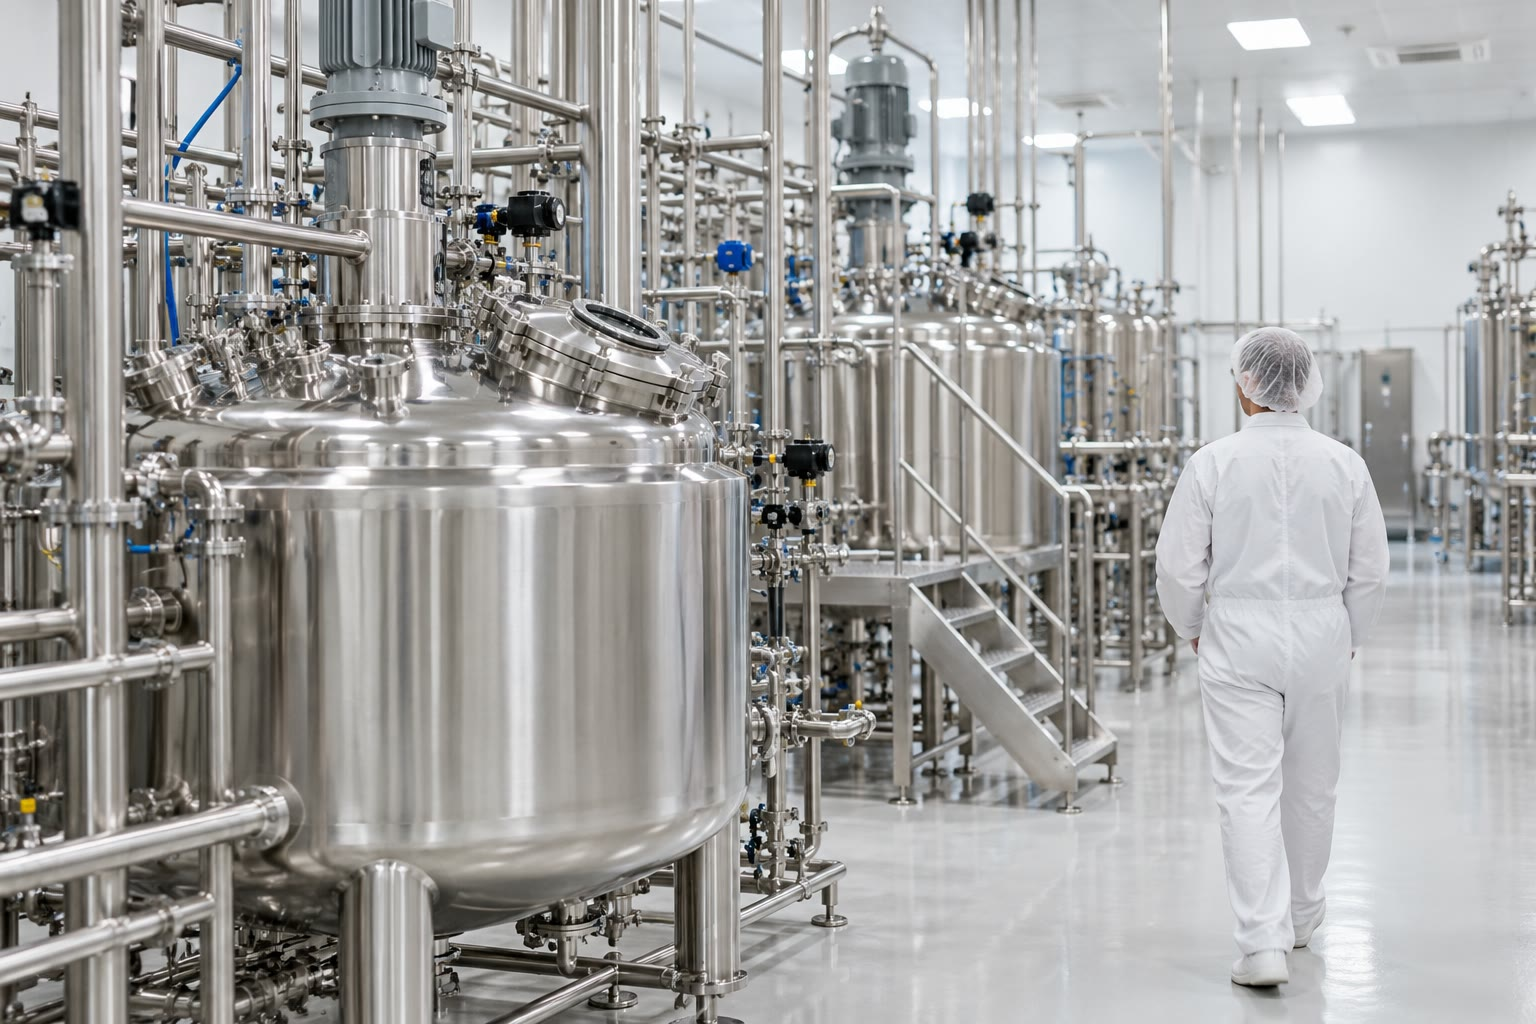
\includegraphics[width=0.48\linewidth]{images/book1/ai/g12-pharma-plant.jpg}

{\small Pabrik farmasi: reaktor-reaktor sebuah \omterm{def:g10:synthesis-yield:synthesis}{sintesis}, yang
diperbesar sampai skala ton.}
\end{omfigure}

\section{Mengoptimalkan sintesis}

Dua hal yang berbeda dapat ditingkatkan: \emph{laju}, yang menentukan
berapa lama \omterm{def:g10:synthesis-yield:synthesis}{sintesis} berlangsung, dan \emph{\omterm{def:g10:synthesis-yield:yield}{rendemen}}, yang menentukan
berapa banyak produk yang dihasilkannya.

\begin{proposition}[Pengungkit laju dan rendemen]\label{prop:g12:synthesis-strategy:levers}
\begin{itemize}
  \item Laju naik dengan suhu, dengan konsentrasi \omterm{def:g7:chemical-reactions:reactant}{pereaksi}, dan dengan
        \omterm{def:g12:catalysis:catalyst}{katalis}.
  \item \omterm{def:g10:synthesis-yield:yield}{Rendemen} akhir \omterm{def:g10:reaction-progress-table:limiting}{reaksi tuntas} ditentukan oleh \omterm{def:g10:reaction-progress-table:limiting}{pereaksi pembatas};
        \omterm{def:g10:synthesis-yield:yield}{rendemen} \omterm{def:g12:equilibrium:non-total}{reaksi tidak tuntas} naik dengan salah satu \omterm{def:g7:chemical-reactions:reactant}{pereaksi}
        yang berlebih, atau dengan pengambilan sebuah produk selagi
        terbentuk. \omterm{def:g12:catalysis:catalyst}{Katalis} tidak mengubahnya: \omterm{def:g12:catalysis:catalyst}{katalis} hanya membawa
        sistem lebih cepat ke \omterm{def:g10:reaction-progress-table:system}{keadaan akhir} yang sama.
\end{itemize}
\end{proposition}

\begin{proof}
Butir pertama menghimpun faktor-faktor kinetik dalam
\cref{ch:g12:reaction-rates,ch:g12:catalysis}. Butir kedua mengikuti dari
$Q = K$ pada akhir \omterm{def:g12:equilibrium:non-total}{reaksi tidak tuntas}: menambahkan \omterm{def:g7:chemical-reactions:reactant}{pereaksi} atau
mengambil produk membuat $Q < K$, dan reaksinya terus berlangsung ke
arah maju.
\end{proof}

\begin{example}[Esterifikasi dengan perangkap air]\label{ex:g12:synthesis-strategy:trap}
Asam etanoat dan etanol, masing-masing satu \omterm{def:g10:the-mole:amount}{mol}, hanya menghasilkan
\qty{67}{\percent} \omterm{def:g11:functional-groups:carboxylic-acid}{ester} pada kesetimbangan. Jika \omterm{def:g6:pure-substances-and-mixtures:mixture}{campurannya} dipanaskan
dengan refluks dalam \omterm{def:g6:solutions-and-solubility:solute}{pelarut} yang tidak bercampur dengan air, dengan
sedikit asam sebagai \omterm{def:g12:catalysis:catalyst}{katalis}, uapnya mengembun ke dalam tabung samping,
sebuah \emph{perangkap air}: air, yang lebih rapat, mengendap di dasar
dan tetap di sana, sementara \omterm{def:g6:solutions-and-solubility:solute}{pelarutnya} mengalir kembali ke dalam labu.
Air meninggalkan reaksi selagi terbentuk, $Q$ tetap di bawah $K$, dan
esterifikasinya hampir tuntas. Pemanasan memberikan laju, \omterm{def:g12:catalysis:catalyst}{katalis}
menambah laju, perangkap memberikan \omterm{def:g10:synthesis-yield:yield}{rendemen}.
\end{example}

\begin{omfigure}
\begin{tikzpicture}[font=\small, scale=0.8]
  \pic[transform shape] at (0,0) {hotplate};
  \pic[transform shape] at (0,0) {rbflask={0.55}{orange!20}};
  % the trap: water at the bottom, solvent above, up to the arm
  \fill[cyan!60!blue!40] (1.0,1.75) arc[start angle=180, end angle=360, radius=0.15] -- (1.3,2.3) -- (1.0,2.3) -- cycle;
  \fill[yellow!35] (1.0,2.3) rectangle (1.3,3.25);
  \draw[om glass] (-0.2,3.0) -- (-0.2,3.75) -- (0.2,3.75) -- (0.2,3.55) -- (1.0,3.55) -- (1.0,4.0);
  \draw[om glass] (0.2,3.0) -- (0.2,3.25) -- (1.0,3.25) -- (1.0,1.75) arc[start angle=180, end angle=360, radius=0.15] -- (1.3,4.0);
  \pic[transform shape] at (1.15,4.0) {condenser};
  \draw[omProp, thick, <-] (1.35,2.0) -- (2.6,1.7) node[right, text=black, align=left] {air terkumpul\\ di dasar};
  \draw[omProp, thick, <-] (1.35,2.9) -- (2.6,3.1) node[right, text=black, align=left] {pelarut meluap\\ kembali ke labu};
  \draw[omProp, thick, <-] (-0.6,0.6) -- (-1.7,1.1) node[left, text=black, align=right] {asam, alkohol,\\ katalis, pelarut};
\end{tikzpicture}

{\small Perangkap air pada labu yang dipanaskan dengan refluks: air yang
terbentuk diambil dari reaksi selagi mengembun.}
\end{omfigure}

\section{Selektivitas}

\omterm{def:g7:atoms-and-molecules:molecule}{Molekul} nyata sering membawa beberapa \omterm{def:g11:functional-groups:functional-group}{gugus fungsi}. \omterm{def:g7:identifying-substances:characteristic-test}{Reagen} yang
menyerang semuanya menghasilkan \omterm{def:g6:pure-substances-and-mixtures:mixture}{campuran}; \omterm{def:g10:synthesis-yield:synthesis}{sintesis} yang baik memakai
\omterm{def:g7:identifying-substances:characteristic-test}{reagen} yang hanya menyerang gugus yang akan diubah.

\begin{definition}[Reaksi kemoselektif]\label{def:g12:synthesis-strategy:chemoselective}
Sebuah reaksi disebut \emph{kemoselektif}\index{reaksi kemoselektif}
jika, pada \omterm{def:g7:atoms-and-molecules:molecule}{molekul} yang membawa beberapa \omterm{def:g11:functional-groups:functional-group}{gugus fungsi}, \omterm{def:g7:identifying-substances:characteristic-test}{reagennya}
mengubah satu gugus dan membiarkan gugus lainnya tidak berubah.
\end{definition}

\begin{example}[Reduktor yang memilih]\label{ex:g12:synthesis-strategy:nabh4}
Natrium borohidrida, \ce{NaBH4}, mereduksi gugus karbonil \omterm{def:g11:functional-groups:carbonyl}{aldehida} dan
\omterm{def:g11:functional-groups:carbonyl}{keton} menjadi gugus \omterm{def:g11:functional-groups:alcohol}{alkohol}, tetapi tidak menyentuh \omterm{def:g11:functional-groups:carboxylic-acid}{ester}. Pada \omterm{def:g7:atoms-and-molecules:molecule}{molekul}
yang membawa sebuah \omterm{def:g11:functional-groups:carbonyl}{keton} dan sebuah \omterm{def:g11:functional-groups:carboxylic-acid}{ester}, hanya \omterm{def:g11:functional-groups:carbonyl}{ketonnya} yang
berubah:
\[
  \ce{CH3-CO-CH2-CH2-CO-O-CH3}
  \;\xrightarrow{\ \ce{NaBH4}\ }\;
  \ce{CH3-CH(OH)-CH2-CH2-CO-O-CH3} .
\]
\omterm{def:g11:redox:oxidant}{Reduktor} yang lebih kuat, litium aluminium hidrida \ce{LiAlH4}, akan
mereduksi kedua gugus: \omterm{def:g11:redox:oxidant}{reduktor} itu tidak \omterm{def:g12:synthesis-strategy:chemoselective}{kemoselektif} di sini.
\end{example}

\begin{remark}[Beberapa jenis selektivitas]\label{rem:g12:synthesis-strategy:kinds}
Kemoselektivitas memilih di antara gugus-gugus. Sebuah reaksi juga dapat
memilih di antara dua posisi pada gugus yang sama, atau di antara dua
\omterm{def:g12:stereochemistry:stereoisomer}{stereoisomer} produknya, seperti yang diperlihatkan \omterm{def:g12:catalysis:enzyme}{enzim-enzim} dalam
\cref{ch:g12:catalysis} dan \omterm{def:g7:atoms-and-molecules:molecule}{molekul-molekul} \omterm{def:g12:stereochemistry:chiral}{kiral} dalam
\cref{ch:g12:stereochemistry}. Setiap jenis selektivitas dipelajari
dalam buku-buku universitas.
\end{remark}

\section{Gugus pelindung}

Jika tidak ada \omterm{def:g7:identifying-substances:characteristic-test}{reagen} yang cukup selektif, ahli kimia menyembunyikan
gugus yang tidak boleh bereaksi, menjalankan reaksinya, lalu membuka
kembali gugus itu.

\begin{definition}[Gugus pelindung]\label{def:g12:synthesis-strategy:protecting-group}
Yang disebut \emph{gugus pelindung}\index{gugus pelindung} adalah gugus
yang dipasang pada sebuah \omterm{def:g11:functional-groups:functional-group}{gugus fungsi} untuk mencegahnya bereaksi
selama satu atau beberapa tahap \omterm{def:g10:synthesis-yield:synthesis}{sintesis}, lalu dilepas sesudahnya untuk
mengembalikan gugus semula. Ketiga operasinya adalah
\emph{proteksi}, \emph{reaksi}, dan \emph{deproteksi}.
\end{definition}

\begin{method}[Merencanakan proteksi]\label{met:g12:synthesis-strategy:plan}
\begin{enumerate}
  \item Daftarlah gugus-gugus setiap \omterm{def:g7:chemical-reactions:reactant}{pereaksi}, serta satu ikatan yang
        akan dibuat.
  \item Tandai setiap gugus lain yang juga dapat diserang oleh \omterm{def:g7:identifying-substances:characteristic-test}{reagen}
        pada tahap itu.
  \item Lindungilah masing-masing dengan gugus yang tahan terhadap
        kondisi reaksi dan dapat dilepas dalam kondisi lunak yang
        membiarkan ikatan baru itu utuh.
  \item Hitunglah biayanya: setiap proteksi menambah dua tahap, proteksi
        dan deproteksi, dan menurunkan \omterm{def:g10:synthesis-yield:yield}{rendemen} keseluruhan.
\end{enumerate}
\end{method}

\begin{example}[Membuat satu dipeptida, bukan empat]\label{ex:g12:synthesis-strategy:dipeptide}
Glisina, \ce{H2N-CH2-COOH}, dan alanina, \ce{H2N-CH(CH3)-COOH},
masing-masing membawa gugus \omterm{def:g11:functional-groups:amine}{amina} dan gugus asam. Ikatan \omterm{def:g11:functional-groups:amine}{amida} antara
asam glisina dan \omterm{def:g11:functional-groups:amine}{amina} alanina menghasilkan dipeptida Gly--Ala. Jika
\omterm{def:g2:mixing-and-dissolving:mix}{dicampur} langsung, kedua asam amino itu menghasilkan empat dipeptida,
Gly--Ala, Ala--Gly, Gly--Gly, dan Ala--Ala, dalam \omterm{def:g6:pure-substances-and-mixtures:mixture}{campuran} yang sulit
dipisahkan. Rencananya:
\begin{enumerate}
  \item lindungi \omterm{def:g11:functional-groups:amine}{amina} glisina dengan gugus yang ditulis \ce{Z}, dan
        asam alanina sebagai \omterm{def:g11:functional-groups:carboxylic-acid}{ester} metilnya;
  \item bentuklah ikatan \omterm{def:g11:functional-groups:amine}{amida}: hanya tersisa satu gugus asam dan satu
        gugus \omterm{def:g11:functional-groups:amine}{amina} yang bebas;
  \item lepaskan kedua \omterm{def:g12:synthesis-strategy:protecting-group}{gugus pelindung}.
\end{enumerate}
\end{example}

\begin{omfigure}
\begin{tikzpicture}[font=\small, node distance=0.55cm,
    box/.style={draw=omDef, rounded corners=2pt, fill=omDef!6, align=center, inner sep=4pt}]
  \node[box] (a) {\ce{H2N-CH2-COOH}\\ \ce{H2N-CH(CH3)-COOH}};
  \node[box, below=of a] (b) {\ce{Z-NH-CH2-COOH}\\ \ce{H2N-CH(CH3)-CO-O-CH3}};
  \node[box, below=of b] (c) {\ce{Z-NH-CH2-CO-NH-CH(CH3)-CO-O-CH3}};
  \node[box, below=of c] (d) {\ce{H2N-CH2-CO-NH-CH(CH3)-COOH}};
  \draw[->, thick, omProp] (a) -- node[right, xshift=3pt, text=black] {1. proteksi} (b);
  \draw[->, thick, omProp] (b) -- node[right, xshift=3pt, text=black] {2. reaksi: ikatan amida} (c);
  \draw[->, thick, omProp] (c) -- node[right, xshift=3pt, text=black] {3. deproteksi} (d);
  \node[anchor=east, font=\footnotesize, text=black!70] at ([xshift=-6pt]a.west) {glisina, alanina};
  \node[anchor=east, font=\footnotesize, text=black!70] at ([xshift=-6pt]d.west) {Gly--Ala};
\end{tikzpicture}

{\small Proteksi, reaksi, deproteksi: satu-satunya ikatan \omterm{def:g11:functional-groups:amine}{amida} yang
dapat terbentuk adalah ikatan yang diinginkan.}
\end{omfigure}

\section{Ekonomi atom}

\omterm{def:g10:synthesis-yield:yield}{Rendemen} \qty{100}{\percent} menyatakan bahwa setiap \omterm{def:g7:atoms-and-molecules:molecule}{molekul} \omterm{def:g10:reaction-progress-table:limiting}{pereaksi
pembatas} menjadi produk. \omterm{def:g10:synthesis-yield:yield}{Rendemen} tidak menyatakan berapa banyak \omterm{def:g7:atoms-and-molecules:atom}{atom}
yang dibeli berakhir di dalam produk: produk-produk lain dalam
persamaan, semurni apa pun, adalah limbah kecuali ada yang dapat
memakainya.

\begin{definition}[Ekonomi atom]\label{def:g12:synthesis-strategy:atom-economy}
Yang disebut \emph{ekonomi atom}\index{ekonomi atom} sebuah \omterm{def:g10:synthesis-yield:synthesis}{sintesis}
adalah bagian dari massa \omterm{def:g7:chemical-reactions:reactant}{pereaksi}, yang diambil dengan perbandingan
dalam \omterm{def:g8:balanced-equations:equation}{persamaan setara}, yang berakhir di dalam produk yang diinginkan.
\end{definition}

\begin{proposition}[Ekonomi atom dari persamaan]\label{prop:g12:synthesis-strategy:atom-economy}
Untuk \omterm{def:g8:balanced-equations:equation}{persamaan setara} $a_1\,\ce{R1} + a_2\,\ce{R2} + \cdots \rightarrow
p\,\ce{P} + \text{produk lain}$,
\[
  \text{ekonomi atom} =
  \frac{p\,M(\ce{P})}{a_1 M(\ce{R1}) + a_2 M(\ce{R2}) + \cdots}
  \times 100\,\% .
\]
\end{proposition}

\begin{proof}
Untuk $x$ \omterm{def:g10:the-mole:amount}{mol} reaksi, massa \omterm{def:g7:chemical-reactions:reactant}{pereaksi} yang terpakai adalah
$x\,(a_1 M(\ce{R1}) + \cdots)$ dan massa produk yang diinginkan yang
terbentuk adalah $x\,p\,M(\ce{P})$; perbandingan keduanya tidak
bergantung pada $x$.
\end{proof}

\begin{method}[Menghitung ekonomi atom]\label{met:g12:synthesis-strategy:atom-economy}
\begin{enumerate}
  \item Tuliskan \omterm{def:g8:balanced-equations:equation}{persamaan setaranya}; untuk jalur dengan beberapa tahap,
        jumlahkan tahap-tahapnya sehingga setiap zat antara saling
        meniadakan.
  \item Hitung \omterm{def:g10:the-mole:molar-mass}{massa molar} setiap \omterm{def:g7:chemical-reactions:reactant}{pereaksi} dan \omterm{def:g10:the-mole:molar-mass}{massa molar} produk yang
        diinginkan.
  \item Terapkan rumusnya, dengan \omterm{def:g8:balanced-equations:coefficient}{koefisien stoikiometrinya}.
  \item Limbah per kilogram produk adalah
        $(100 - \text{ekonomi atom})/\text{ekonomi atom}$ kilogram.
\end{enumerate}
\end{method}

\begin{example}[Adisi dibandingkan substitusi]\label{ex:g12:synthesis-strategy:compare}
% ledger: aw:C, aw:H, aw:Br, aw:Na, aw:O
Bromoetana dari etena, \ce{C2H4 + HBr -> C2H5Br}: setiap \omterm{def:g7:atoms-and-molecules:atom}{atom} berakhir
di dalam produk, \omterm{def:g12:synthesis-strategy:atom-economy}{ekonomi atom} $108.9/(28.0 + 80.9) = \qty{100}{\percent}$.
Etanol dari bromoetana, \ce{C2H5Br + NaOH -> C2H5OH + NaBr}: \omterm{def:g12:synthesis-strategy:atom-economy}{ekonomi
atomnya} $46.0/(108.9 + 40.0) = \qty{30.9}{\percent}$; per kilogram
etanol, terbentuk \qty{2.2}{kg} natrium bromida. \omterm{def:g12:curly-arrows:categories}{Adisi} selalu memiliki
\omterm{def:g12:synthesis-strategy:atom-economy}{ekonomi atom} \qty{100}{\percent}; \omterm{def:g12:curly-arrows:categories}{substitusi} atau \omterm{def:g12:curly-arrows:categories}{eliminasi} tidak pernah.
\end{example}

\begin{omfigure}
\begin{tikzpicture}
\begin{axis}[width=0.8\linewidth, height=5.2cm, ybar, bar width=16pt,
    ymin=0, ymax=112, ylabel={ekonomi atom (\%)},
    xtick={1,2,3,4,5}, xticklabels={adisi, esterifikasi, ibuprofen (3 tahap), ibuprofen (6 tahap), substitusi},
    xticklabel style={font=\footnotesize, align=center, text width=2.1cm},
    nodes near coords, nodes near coords style={font=\footnotesize},
    enlarge x limits=0.12, axis lines*=left, ymajorgrids, grid style={black!12}]
  \addplot[fill=omDef!55, draw=omDef] table[x=i, y=AE] {figdata/out/grade-12-synthesis-strategy.dat};
\end{axis}
\end{tikzpicture}

{\small \omterm{def:g12:synthesis-strategy:atom-economy}{Ekonomi atom} yang dihitung dari persamaan: etena dengan hidrogen
bromida, asam etanoat dengan etanol, kedua jalur ibuprofen, dan
bromoetana dengan natrium hidroksida.}
\end{omfigure}

\section{Kimia hijau}

\begin{definition}[Kimia hijau]\label{def:g12:synthesis-strategy:green-chemistry}
Yang disebut \emph{kimia hijau}\index{kimia hijau} adalah perancangan
produk dan proses kimia yang mengurangi atau meniadakan penggunaan dan
pembentukan zat berbahaya, dari pemilihan bahan awal sampai nasib produk
setelah dipakai.
\end{definition}

Dua belas prinsip merangkum pendekatan ini; setiap prinsip adalah
pertanyaan yang perlu diajukan pada sebuah proses.
% ledger: green:12
\begin{enumerate}
  \item Cegah limbah daripada mengolahnya.
  \item Maksimalkan \omterm{def:g12:synthesis-strategy:atom-economy}{ekonomi atom}.
  \item Rancang \omterm{def:g10:synthesis-yield:synthesis}{sintesis} yang kurang berbahaya.
  \item Rancang bahan kimia dan produk yang lebih aman.
  \item Pakai \omterm{def:g6:solutions-and-solubility:solute}{pelarut} dan kondisi reaksi yang lebih aman.
  \item Tingkatkan efisiensi energi: bekerjalah pada suhu dan tekanan
        yang dekat dengan suhu dan tekanan kamar.
  \item Pakai \omterm{def:g5:raw-materials-and-recycling:raw-material}{bahan baku} terbarukan.
  \item Hindari turunan kimia, seperti \omterm{def:g12:synthesis-strategy:protecting-group}{gugus pelindung}.
  \item Pakai \omterm{def:g12:catalysis:catalyst}{katalis}, bukan \omterm{def:g7:identifying-substances:characteristic-test}{reagen} stoikiometris.
  \item Rancang produk yang terurai setelah dipakai.
  \item Lakukan analisis seketika untuk mencegah pencemaran.
  \item Perkecil kemungkinan terjadinya kecelakaan.
\end{enumerate}

\begin{remark}[Prinsip, bukan hukum]\label{rem:g12:synthesis-strategy:principles}
Prinsip-prinsip itu sering saling tarik ke arah yang berlawanan: \omterm{def:g12:synthesis-strategy:protecting-group}{gugus
pelindung} melanggar prinsip 8 tetapi dapat menyelamatkan seluruh
\omterm{def:g10:synthesis-yield:synthesis}{sintesis}; \omterm{def:g12:catalysis:catalyst}{katalis} yang menghemat energi dapat mengandung \omterm{def:g9:periodic-table-first-look:metal}{logam} yang
langka. Menilai sebuah proses berarti menimbang prinsip-prinsip itu,
dengan angka sedapat mungkin: \omterm{def:g12:synthesis-strategy:atom-economy}{ekonomi atom}, \omterm{def:g10:synthesis-yield:yield}{rendemen}, massa limbah,
energi.
\end{remark}

\begin{history}[Kimia hijau, 1998]
% ledger: green:book-1998, ibu:bhc-commercial
Pada tahun 1998 ahli kimia Paul Anastas dan John Warner menerbitkan
sebuah buku, \emph{Green Chemistry: Theory and Practice}, yang
memaparkan kedua belas prinsip itu. Setahun sebelumnya, sebuah
penghargaan pemerintah untuk \omterm{def:g10:synthesis-yield:synthesis}{sintesis} yang lebih hijau diberikan kepada
jalur tiga tahap pembuatan ibuprofen, yang telah dijalankan dalam skala
industri sejak 1992. Sejak itu, prinsip-prinsip tersebut diajarkan
kepada para ahli kimia sebagai bagian dari keahlian mereka.
\end{history}

\begin{example}[Dua jalur menuju ibuprofen]\label{ex:g12:synthesis-strategy:ibuprofen}
% ledger: ibu:boots-steps, ibu:bhc-steps, ibu:boots-ae, ibu:bhc-ae, ibu:bhc-ae-recovered
Ibuprofen, \ce{C13H18O2}, dibuat dari hidrokarbon \ce{C10H14}
(isobutilbenzena). Jalur yang lebih tua memakai enam tahap dan, pada
setiap tahap, \omterm{def:g7:identifying-substances:characteristic-test}{reagen} dalam jumlah penuh; jika dijumlahkan, \omterm{def:g10:the-mole:molar-mass}{massa molar}
seluruh \omterm{def:g7:chemical-reactions:reactant}{pereaksinya} \qty{514.5}{g/mol}, untuk \qty{206.0}{g/mol}
ibuprofen: \omterm{def:g12:synthesis-strategy:atom-economy}{ekonomi atom} \qty{40}{\percent}. Jalur yang lebih baru
memakai tiga tahap, dua di antaranya dengan \omterm{def:g12:catalysis:catalyst}{katalis}, dan persamaan
keseluruhannya
\[
  \ce{C10H14 + C4H6O3 + H2 + CO -> C13H18O2 + C2H4O2}
\]
memberikan $206.0/266.0 = \qty{77}{\percent}$. Hasil sampingnya, asam
etanoat, diambil kembali dan dipakai: jika dihitung sebagai produk,
\omterm{def:g12:synthesis-strategy:atom-economy}{ekonomi atomnya} melebihi \qty{99}{\percent}.
\end{example}

\begin{omfigure}
\chemfig{[:30]*6(-=(-[:90](-[:150])-[:30](=[:90]O)-[:-30]OH)-=-(-[:-90]-[:-150](-[:150])-[:-90])=)}

\medskip
\begin{tikzpicture}[font=\scriptsize,
    st/.style={draw=omDef, rounded corners=2pt, fill=omDef!6, minimum height=0.8cm, text width=1.15cm, align=center, inner sep=2pt}]
  \foreach \i/\t in {1/asilasi, 2/+ 2 karbon, 3/aldehida, 4/oksim, 5/nitril, 6/asam}
    \node[st] (o\i) at (1.7*\i,0) {\t};
  \foreach \i/\j in {1/2,2/3,3/4,4/5,5/6} \draw[->, thick] (o\i) -- (o\j);
  \node[anchor=east, align=right, font=\footnotesize] at ([xshift=-4pt]o1.west) {6 tahap\\ \textbf{40 \%}};
  \foreach \i/\t in {1/asilasi, 2/adisi \ce{H2}, 3/adisi \ce{CO}}
    \node[st, fill=omProp!8, draw=omProp] (n\i) at (1.7*\i,-1.4) {\t\\ (katalis)};
  \foreach \i/\j in {1/2,2/3} \draw[->, thick] (n\i) -- (n\j);
  \node[anchor=east, align=right, font=\footnotesize] at ([xshift=-4pt]n1.west) {3 tahap\\ \textbf{77 \%}};
  \node[anchor=west, align=left, font=\footnotesize] at ([xshift=6pt]n3.east) {hasil samping: asam etanoat, diambil kembali;\\ jika dihitung sebagai produk: lebih dari 99 \%};
\end{tikzpicture}

{\small Ibuprofen (atas) dan kedua jalur industrinya: yang lebih tua,
enam tahap, dan yang lebih baru, tiga tahap dengan \omterm{def:g12:catalysis:catalyst}{katalis}, beserta
\omterm{def:g12:synthesis-strategy:atom-economy}{ekonomi atomnya}.}
\end{omfigure}

\begin{example}[Pelarut yang lebih hijau]\label{ex:g12:synthesis-strategy:solvents}
% ledger: crit:CO2-T, crit:CO2-p
Banyak reaksi dan \omterm{def:g10:chemical-species:extraction}{ekstraksi} memakai \omterm{def:g6:solutions-and-solubility:solute}{pelarut} organik yang beracun, mudah
menyala, atau mudah \omterm{def:g3:separating-mixtures:evaporate}{menguap}. Air adalah \omterm{def:g6:solutions-and-solubility:solute}{pelarut} yang paling aman, jika
\omterm{def:g7:chemical-reactions:reactant}{pereaksinya} \omterm{def:g2:mixing-and-dissolving:dissolve}{larut} di dalamnya. Karbon dioksida menjadi \omterm{def:g6:solutions-and-solubility:solute}{pelarut} lain: di
atas \qty{31}{\celsius} dan \qty{73.8}{bar}, zat itu menjadi
\emph{fluida superkritis}, bukan cairan dan bukan gas, yang melarutkan
banyak \omterm{def:g7:atoms-and-molecules:molecule}{molekul} organik. Fluida ini mengekstraksi kafein dari biji kopi,
misalnya; ketika tekanannya dilepaskan, fluida itu begitu saja kembali
menjadi gas dan tidak meninggalkan residu dalam produk.
\end{example}

\begin{omfigure}
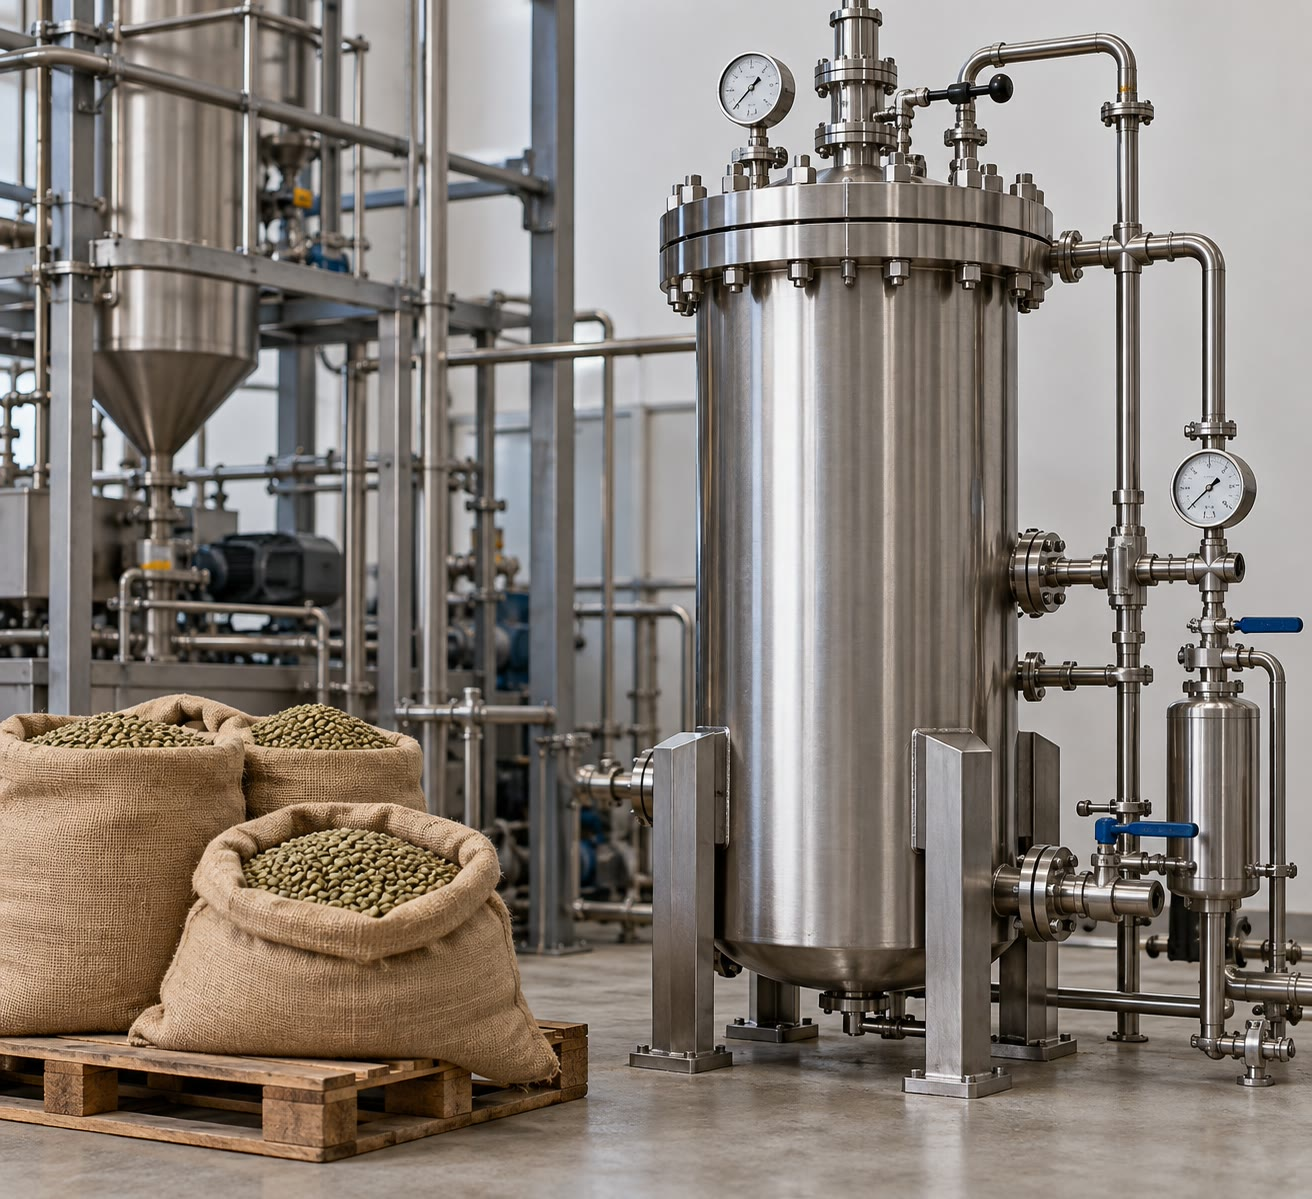
\includegraphics[width=0.45\linewidth,height=6cm,keepaspectratio]{images/book1/ai/g12-scco2-vessel.jpg}

{\small Bejana \omterm{def:g10:chemical-species:extraction}{ekstraksi} bertekanan tinggi, tempat karbon dioksida
superkritis menggantikan \omterm{def:g6:solutions-and-solubility:solute}{pelarut} organik.}
\end{omfigure}

\section{Latihan}

\begin{exercise}[$\star$]\label{exo:g12:synthesis-strategy:1}
Etanol dapat dibuat dengan hidrasi etena, \ce{C2H4 + H2O -> C2H5OH},
atau dengan fermentasi glukosa, \ce{C6H12O6 -> 2C2H5OH + 2CO2}. Hitung
\omterm{def:g12:synthesis-strategy:atom-economy}{ekonomi atom} masing-masing.
\end{exercise}

\begin{exercise}[$\star$]\label{exo:g12:synthesis-strategy:2}
Pada skema dipeptida dalam bab ini, sebutkan tahap tempat setiap \omterm{def:g12:synthesis-strategy:protecting-group}{gugus
pelindung} dipasang, dan tahap tempat gugus itu dilepas.
\end{exercise}

\begin{exercise}[$\star$]\label{exo:g12:synthesis-strategy:3}
Sebuah pabrik mengganti \omterm{def:g6:solutions-and-solubility:solute}{pelarut} terklorinasi dengan air dalam salah satu
reaksinya. Prinsip \omterm{def:g12:synthesis-strategy:green-chemistry}{kimia hijau} mana yang diterapkannya?
\end{exercise}

\begin{exercise}[$\star$]\label{exo:g12:synthesis-strategy:4}
Mengapa etanol berlebih menaikkan \omterm{def:g10:synthesis-yield:yield}{rendemen} esterifikasi, sedangkan
\omterm{def:g12:catalysis:catalyst}{katalis} tidak?
\end{exercise}

\begin{exercise}[$\star$]\label{exo:g12:synthesis-strategy:5}
Natrium borohidrida mereduksi \omterm{def:g11:functional-groups:carbonyl}{aldehida} dan \omterm{def:g11:functional-groups:carbonyl}{keton}, bukan \omterm{def:g11:functional-groups:carboxylic-acid}{ester}. Apakah
reaksinya dengan metil 4-oksopentanoat (sebuah \omterm{def:g11:functional-groups:carbonyl}{keton} dan sebuah \omterm{def:g11:functional-groups:carboxylic-acid}{ester})
\omterm{def:g12:synthesis-strategy:chemoselective}{kemoselektif}? Gugus mana yang berubah?
\end{exercise}

\begin{exercise}[$\star\star$]\label{exo:g12:synthesis-strategy:6}
Satu \omterm{def:g10:the-mole:amount}{mol} asam etanoat dan satu \omterm{def:g10:the-mole:amount}{mol} etanol menghasilkan \qty{0.67}{mol}
\omterm{def:g11:functional-groups:carboxylic-acid}{ester} pada kesetimbangan. Usulkan dua cara untuk menaikkan jumlah ini,
dan satu cara untuk mencapainya lebih cepat.
\end{exercise}

\begin{exercise}[$\star\star$]\label{exo:g12:synthesis-strategy:7}
Metil 4-oksopentanoat, \ce{CH3-CO-CH2-CH2-CO-O-CH3}, direaksikan sekali
dengan natrium borohidrida, dan sekali lagi dengan litium aluminium
hidrida berlebih, yang mereduksi \omterm{def:g11:functional-groups:carboxylic-acid}{ester} menjadi dua \omterm{def:g11:functional-groups:alcohol}{alkohol}. Tuliskan
setiap produknya.
\end{exercise}

\begin{exercise}[$\star\star$]\label{exo:g12:synthesis-strategy:8}
Pada diagram batang \omterm{def:g12:synthesis-strategy:atom-economy}{ekonomi atom}, reaksi mana yang mempertahankan lebih
dari tiga perempat \omterm{def:g7:atoms-and-molecules:atom}{atomnya}? Dengan faktor berapa jalur tiga tahap menuju
ibuprofen lebih baik daripada jalur enam tahap?
\end{exercise}

\begin{exercise}[$\star\star$]\label{exo:g12:synthesis-strategy:9}
Aspirin dibuat dengan \ce{C7H6O3 + C4H6O3 -> C9H8O4 + C2H4O2}. Hitung
\omterm{def:g12:synthesis-strategy:atom-economy}{ekonomi atomnya} dan massa hasil samping per kilogram aspirin.
\end{exercise}

\begin{exercise}[$\star\star$]\label{exo:g12:synthesis-strategy:10}
Mengapa \omterm{def:g10:synthesis-yield:synthesis}{sintesis} dipanaskan dengan refluks dan bukan di dalam labu
terbuka? Manakah yang ditingkatkan oleh pemanasan, laju atau \omterm{def:g10:synthesis-yield:yield}{rendemen}?
\end{exercise}

\begin{exercise}[$\star\star$]\label{exo:g12:synthesis-strategy:11}
Pada gambar kedua jalur ibuprofen, hitunglah tahap-tahapnya, lalu
sebutkan prinsip-prinsip \omterm{def:g12:synthesis-strategy:green-chemistry}{kimia hijau} yang diterapkan jalur yang lebih
baru. Berikan tiga.
\end{exercise}

\begin{exercise}[$\star\star\star$]\label{exo:g12:synthesis-strategy:12}
Sebuah \omterm{def:g10:synthesis-yield:synthesis}{sintesis} tiga tahap memiliki \omterm{def:g10:synthesis-yield:yield}{rendemen} \qty{80}{\percent},
\qty{70}{\percent}, dan \qty{90}{\percent}. Hitung \omterm{def:g10:synthesis-yield:yield}{rendemen}
keseluruhannya. Berapa jumlah bahan awal yang diperlukan untuk
memperoleh \qty{0.10}{mol} produk akhir, jika satu \omterm{def:g10:the-mole:amount}{mol} bahan awal paling
banyak menghasilkan satu \omterm{def:g10:the-mole:amount}{mol} produk?
\end{exercise}

\begin{exercise}[$\star\star\star$]\label{exo:g12:synthesis-strategy:13}
Rencanakan \omterm{def:g10:synthesis-yield:synthesis}{sintesis} dipeptida Ala--Gly (asam alanina yang terikat pada
\omterm{def:g11:functional-groups:amine}{amina} glisina): gugus mana yang kamu lindungi, dan berapa tahap yang
diperlukan rencana itu?
\end{exercise}

\begin{exercise}[$\star\star\star$]\label{exo:g12:synthesis-strategy:14}
Sebuah perusahaan menyebut prosesnya ``hijau'' karena memakai \omterm{def:g12:catalysis:catalyst}{katalis}.
Proses itu berjalan pada \qty{250}{\celsius} dalam benzena, sebuah
\omterm{def:g6:solutions-and-solubility:solute}{pelarut} beracun, dan \omterm{def:g12:synthesis-strategy:atom-economy}{ekonomi atomnya} \qty{35}{\percent}. Nilailah
klaim itu, prinsip demi prinsip.
\end{exercise}

\begin{exercise}[$\star\star\star$]\label{exo:g12:synthesis-strategy:15}
Kafein diekstraksi dari biji kopi dengan diklorometana, sebuah \omterm{def:g6:solutions-and-solubility:solute}{pelarut}
terklorinasi yang mudah \omterm{def:g3:separating-mixtures:evaporate}{menguap}, atau dengan karbon dioksida superkritis
pada sekitar \qty{40}{\celsius} dan \qty{100}{bar}. Jelaskan mengapa
karbon dioksida pada kondisi itu superkritis, mengapa diperlukan bejana
yang kuat, dan berikan dua keunggulannya dibandingkan cara pertama.
\end{exercise}

\section{Soal: Dua Jalur Menuju Ibuprofen}

\begin{problem}[{Soal akhir pekan --- berapa limbah yang dihindari jalur
tiga tahap per ton ibuprofen?}]
\label{pb:g12:synthesis-strategy:1}
% ledger: ibu:boots-ae, ibu:bhc-ae, ibu:boots-steps, ibu:bhc-steps, aw:C, aw:H, aw:O, aw:N, aw:Cl, aw:Na
Jalur yang lebih tua menuju ibuprofen \ce{C13H18O2} memerlukan enam
tahap. Jika dijumlahkan, \omterm{def:g7:chemical-reactions:reactant}{pereaksinya} adalah \ce{C10H14}, \ce{C4H6O3},
\ce{C4H7ClO2}, \ce{C2H5ONa}, sebuah asam yang dihitung sebagai
\ce{H3O}, \ce{NH3O}, dan dua \ce{H2O}. Jalur yang lebih baru memerlukan
tiga tahap:
\[
  \ce{C10H14 + C4H6O3 + H2 + CO -> C13H18O2 + C2H4O2} .
\]

\medskip
\noindent\textbf{Bagian I --- Persamaannya.}
\begin{enumerate}
  \item Periksalah bahwa persamaan jalur yang lebih baru setara dalam
        karbon, hidrogen, dan oksigen.
  \item Sebutkan hasil samping jalur yang lebih baru.
  \item Pada jalur yang lebih tua, unsur-unsur mana dari \omterm{def:g7:chemical-reactions:reactant}{pereaksinya} yang
        seluruhnya berakhir di dalam limbah?
  \item Jalur mana yang memakai \omterm{def:g12:catalysis:catalyst}{katalis}? Prinsip mana yang diterapkan
        dengan hal itu?
\end{enumerate}

\medskip
\noindent\textbf{Bagian II --- \omterm{def:g12:synthesis-strategy:atom-economy}{Ekonomi atom}.}
\begin{enumerate}[resume]
  \item Hitung \omterm{def:g10:the-mole:molar-mass}{massa molar} ibuprofen.
  \item Hitung jumlah \omterm{def:g10:the-mole:molar-mass}{massa molar} \omterm{def:g7:chemical-reactions:reactant}{pereaksi} pada jalur yang lebih tua.
  \item Simpulkan \omterm{def:g12:synthesis-strategy:atom-economy}{ekonomi atomnya}.
  \item Hitung jumlah \omterm{def:g10:the-mole:molar-mass}{massa molar} \omterm{def:g7:chemical-reactions:reactant}{pereaksi} pada jalur yang lebih baru.
  \item Simpulkan \omterm{def:g12:synthesis-strategy:atom-economy}{ekonomi atomnya}.
  \item Menjadi berapa \omterm{def:g12:synthesis-strategy:atom-economy}{ekonomi atom} itu jika asam etanoat dihitung
        sebagai produk?
\end{enumerate}

\medskip
\noindent\textbf{Bagian III --- Limbah per ton.}
\begin{enumerate}[resume]
  \item Untuk jalur yang lebih tua, dengan \omterm{def:g10:synthesis-yield:yield}{rendemen} \qty{100}{\percent},
        berapa massa \omterm{def:g7:chemical-reactions:reactant}{pereaksi} yang dibeli per ton ibuprofen?
  \item Berapa massa limbah yang dihasilkannya per ton?
  \item Pertanyaan yang sama untuk jalur yang lebih baru: massa \omterm{def:g7:chemical-reactions:reactant}{pereaksi}
        per ton.
  \item Massa asam etanoat per ton.
  \item Berapa massa limbah per ton yang dihindari jika asam etanoat
        dihitung sebagai limbah?
\end{enumerate}

\medskip
\noindent\textbf{Bagian IV --- \omterm{def:g10:synthesis-yield:yield}{Rendemen} dan dunia nyata.}
\begin{enumerate}[resume]
  \item Andaikan setiap tahap memiliki \omterm{def:g10:synthesis-yield:yield}{rendemen} \qty{90}{\percent}.
        Hitung \omterm{def:g10:synthesis-yield:yield}{rendemen} keseluruhan jalur yang lebih tua.
  \item Sama untuk jalur yang lebih baru.
  \item Berikan satu alasan lagi, selain persamaannya, mengapa tahap
        yang lebih sedikit berarti limbah yang lebih sedikit.
  \item Dalam praktik, asam etanoat diambil kembali dan dipakai. Berapa
        massa limbah per ton yang lalu dihasilkan jalur yang lebih baru,
        dengan \omterm{def:g10:synthesis-yield:yield}{rendemen} \qty{100}{\percent}?
  \item Nyatakan jawaban akhirnya: berapa limbah yang dihindari jalur
        tiga tahap per ton ibuprofen?
\end{enumerate}
\end{problem}
